\begin{frame}{Tìm kiếm lân cận}
  \begin{itemize}
    \item Lân cận
    \item Tối ưu địa phương
    \item Tiêu chí chấp nhận nghiệm
    \item Điều kiện dừng
  \end{itemize}
\end{frame}

\begin{frame}{Tìm kiếm lân cận rộng}
  \begin{figure}[H] % places figure environment here   
    \centering % Centers Graphic
    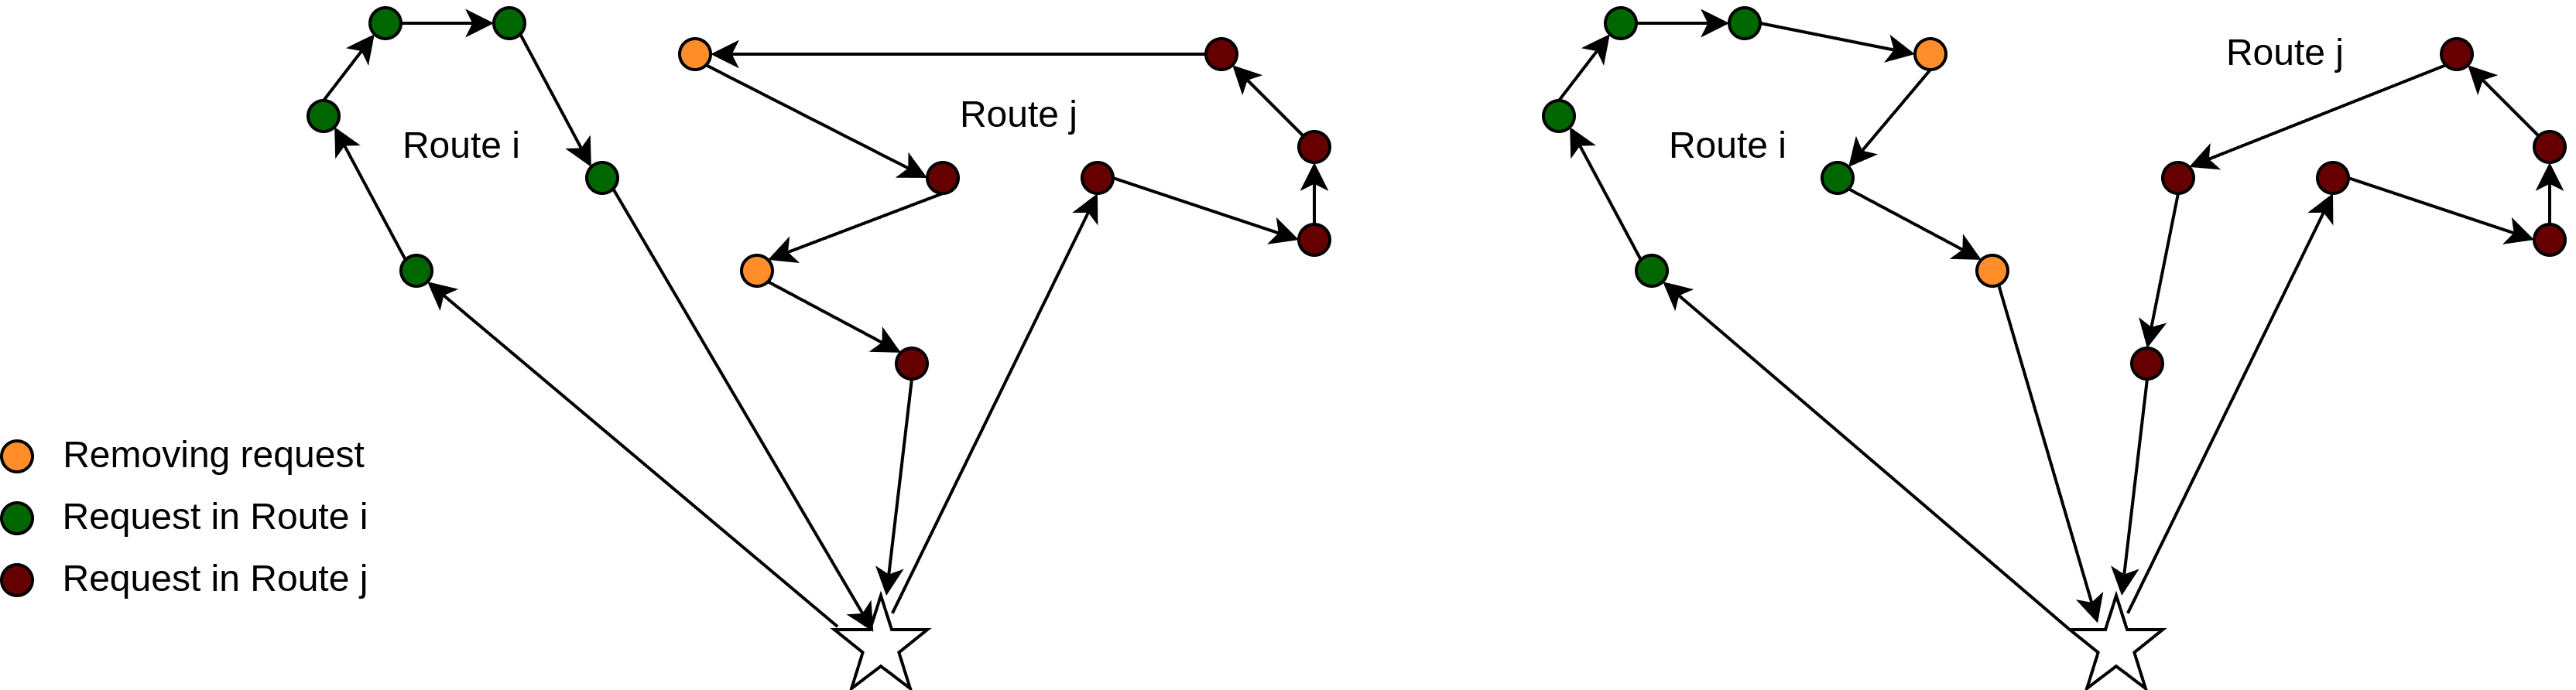
\includegraphics[width=0.9\textwidth]{figures/ALNS-paradim.png} 
    % \includesvg[scale=1]{figures/core-object}
    \caption{Lược đồ LNS} 
    \label{fig:lns_paradim}
  \end{figure}  
\end{frame}

\begin{frame}{Tìm kiếm lân cận rộng (\textit{LNS})}
  \begin{figure}[H] % places figure environment here   
    \centering % Centers Graphic
    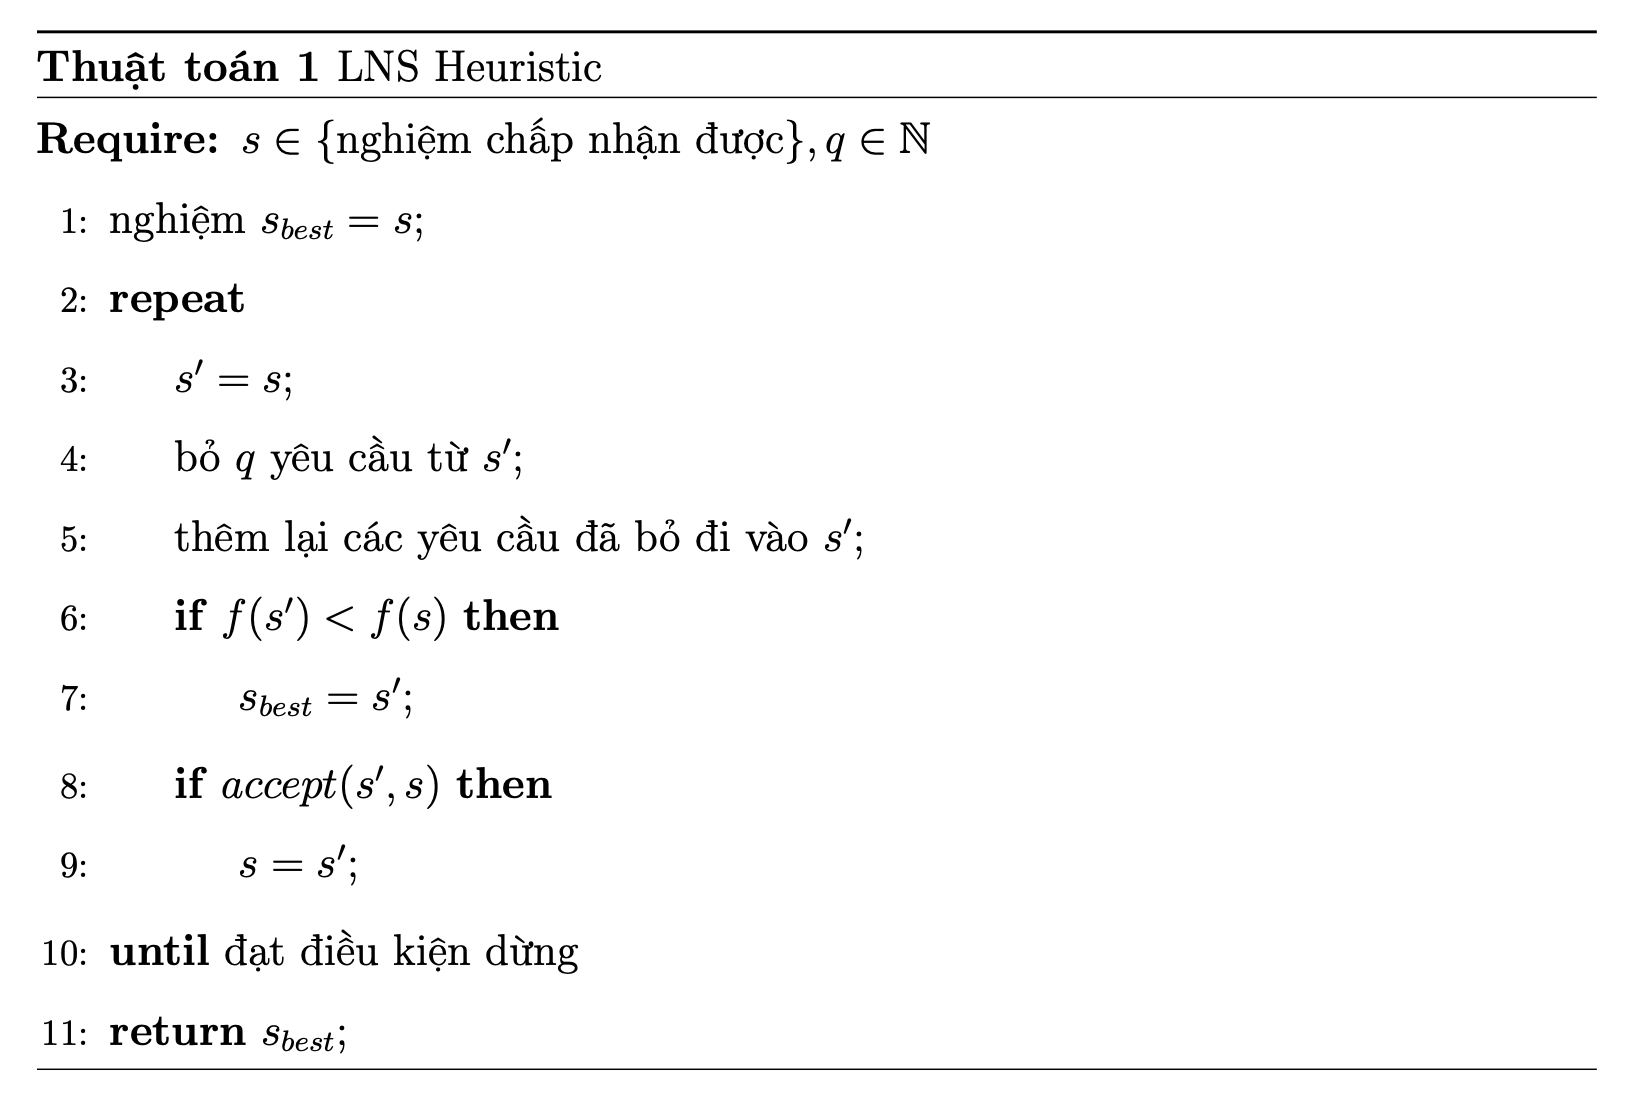
\includegraphics[width=0.8\textwidth]{figures/pr_LNS.png} 
    % \includesvg[scale=1]{figures/core-object}
    \caption{Mã giả LNS} 
    \label{fig:lns_pseudo}
  \end{figure} 
\end{frame}

\begin{frame}{LNS - Thuật toán hủy}
  
\end{frame}

\begin{frame}{LNS - Thuật toán sửa}
  
\end{frame}

\begin{frame}{LNS - Tiêu chí chấp nhận nghiệm}
    \begin{block}{Bước ngẫu nhiên - Ramdom Walk}
      Mọi nghiệm $s'$ đều được chấp nhận.
    \end{block}
    \begin{block}{Chấp nhận tham lam - Greedy Acceptance}
      Nghiệm $s'$ được chấp nhận nếu chi phí của nó là nhỏ hơn so với nghiệm hiện tại.
    \end{block}
    \begin{block}{Mô phỏng luyện kim - Simulated Annealing}
      Mọi nghiệm cải thiện $s'$ được chấp nhận. Nếu $c(s') > c(s)$ thì $s'$ được chấp nhận với xác suất $\exp \{ \frac{c(s) - c(s')}{T} \}$ với $T$ là nhiệt độ. Nhiệt độ $T$ giảm sau mỗi vòng lặp với một hệ số $\Phi$.
    \end{block}
\end{frame}

\begin{frame}{LNS - Tiêu chí chấp nhận nghiệm}
  \begin{block}{Chấp nhận với ngưỡng - Threshold Acceptance}
    Nghiệm $s'$ được chấp nhận nếu $c(s') - c(s) < T$ với $T$ là ngưỡng, ngưỡng này được giảm sau mỗi vòng lặp với hệ số $\Phi$.
  \end{block}
  
  \begin{block}{Đại hồng thủy - Great Deluge Algorithm}
    Nghiệm $s'$ được chấp nhận nếu $c(s') < L$ với một ngưỡng $L$, ngưỡng này chỉ giảm nếu nghiệm được chấp nhận, và giảm với hệ số $\Phi$.
  \end{block}
\end{frame}

\begin{frame}{Tìm kiếm lân cận rộng thích ứng (\textit{ALNS})}
  \begin{block}{Lựa chọn thuật toán hủy và thêm lại}
    Gán cho mỗi heuristic một trọng số khác nhau và sử dụng nguyên tắc "bánh xe lựa chọn". Nếu có $k$ heuristic với trọng số $w_i, i \in \{1,...,k\}$, ta chọn heuristic $j$ với xác suất
    \begin{equation}
      \label{eq:select}
      p_j = \frac{w_j}{\sum_{i=1}^k w_i}.
    \end{equation}
  \end{block}
\end{frame}

\begin{frame}{ALNS - Điều chỉnh tham số tự động}
  \begin{itemize}
    \item Trọng số được điều chỉnh mỗi khi có nghiệm mới được chấp nhận.
    \item Mỗi heuristic được gán điểm khác nhau và được điều chỉnh tùy thuộc vào tình huống.
    \item Cập nhật trọng số sau mỗi bước.
  \end{itemize}
\end{frame}

\begin{frame}{ALNS - Điều chỉnh tham số tự động}
  Điểm của mỗi heuristic được đặt là $0$ khi bắt đầu và được tăng thêm $\sigma_1, \sigma_2, \sigma_3$ tùy thuộc vào tình huống.
  \begin{itemize}
    \justifying
    \item $\sigma_1$ khi hành động xóa-chèn cuối cùng dẫn đến một nghiệm mới tốt hơn nghiệm tốt nhất toàn cục.
    \item $\sigma_2$ khi hành động xóa-chèn cuối cùng dẫn đến một nghiệm chưa được chấp nhận trước đó, chi phí tốt hơn chi phí của nghiệm hiện tại.
    \item $\sigma_3$ khi hành động xóa-chèn cuối cùng dẫn đến một nghiệm chưa được chấp nhận trước đó, chi phí của nghiệm mới tệ hơn chi phí của nghiệm hiện tại nhưng thỏa mãn điều kiện chấp nhận nghiệm.
  \end{itemize}
\end{frame}

\begin{frame}{ALNS - Điều chỉnh tham số tự động}
  $\omega_{ij}$ là trọng số của heuristic $i$ được sử dụng tại bước $j$ \\
  Khi bước $j$ kết thúc, ta tính toán trọng số cho tất cả heuristic $i$ để sử dụng cho bước thứ $j + 1$
  \begin{equation}
      \omega_{i, j+1} = \omega_{ij}(1-r)+r\frac{\pi_i}{\theta_i}.
  \end{equation} \\
  Trong đó, $\pi_i$ là điểm số của heuristic $i$ được nhận trong bước cuối cùng, $\theta_i$ là số lần ta cố gắng sử dụng heuristic $i$ trong bước thực hiện đó, $r$ là tham số điều khiển.
\end{frame}

\begin{frame}{ALNS - B-ALNS}
  \begin{block}{B-ALNS}
    Thêm nhiễu khi điều chỉnh tham số tự động. Giả sử sau $m$ vòng lặp, chúng ta mới lại có một nghiệm được chấp nhận từ lần cuối cùng nghiệm được chấp nhận.
    \begin{equation}
      \label{eq:boost_adaptive_weight}
      \omega_{i, j+1} = \omega_{ij}(1-r)+r\frac{\pi_i} {\theta_i} + \alpha \beta (1 - e^{-\gamma m})
    \end{equation}
    với $\alpha$ (có thể âm hoặc dương) và $\gamma$ (dương) là các tham số điều khiển, $\beta$ là một số ngẫu nhiên trong khoảng $(0,1)$.
  \end{block}
\end{frame}

\begin{frame}{ALNS - Số lượng yêu cầu bỏ đi, thêm lại}
  
\end{frame}

